\section{A Species Distribution analysis using different Machine Learning methods}

The central goal of this task is to predict the different species found at a given set of specified coordinates (latitude, longitude) using a variety of machine learning methods. In our investigation, we analyze the multi-label, classification capabilities of 1.\ \textbf{Logistic Regression}, 2.\ \textbf{Random Forest}, 3.\ \textbf{K-Nearest Neighbour} \& 4.\ \textbf{Feed Forward Neural Network} models. With these four implemented methods we perform subsequent analysis to evaluate and compare the accuracy of each model. Having done so, we aim to answer questions such as the prevalence of specific species in given regions.

\textbf{Logistic Regression} is a simple but powerful linear model for classification which uses a logistic function to model the probability of a binary outcome. This was implemented using the built-in LogisticRegression implementation in scikit-learn. As we wish to study the per-class probabilities at each location, we use the multinomial method, which seeks to minimise the cross-entropy loss during training, rather than a one-versus-rest scheme. The softmax function is then used to calculate the per-class probabilities. The main disadvantage of logistic regression in this context is that the data is unlikely to be linearly separable; for example, if a particular species is distributed across two different continents. Despite this, the ease of implementation for logistic regression makes it an appealing model to study.
\textbf{Random Forests} are a suitable choice for our data-set due to their inherent ability to handle complex data and capture non-linear patterns \cite{breiman2001random}. The ensemble nature of Random Forests is useful to avoid over-fitting and allow for better generalization. Implementation-wise, the model was realized using the scikit-learn library, the number of estimators was set at 100 and the maximum depth was optimized by calculating the F1 scores for different depth values (see Appendix \ref{appendix:RFF1}). At \textit{max\_depth=10}, the performance of the model plateaus and so it was chosen to avoid over-fitting.
\textbf{K-Nearest Neighbours (KNN)} calculates the k-nearest neighbours to a data-point based on some chosen distance metric, then assigns a class based on whichever class makes up the majority of these neighbours. Using sci-kit learn's implementation, we chose $k = 75$ as the number of neighbours, determined by calculating the mean F1 score across all species for different values of $k$ (see Appendix \ref{appendix:KNNF1}). In addition, we use the standard Euclidean metric to determine the distance between points and neighbours. The per-class probabilities for a particular location are calculated as the number of neighbours belonging to each class divided by the total number of neighbours. %We expect KNN to work well for localised species distributions.%
\textbf{Feed-Forward Neural Networks (FFNN's)} are able to implicitly detect non-linear relationships through the use of a connected layer architecture. They are therefore a potentially suitable model to use to train population distributions. They were implemented using PyTorch. A visual of the implementation is provided in Appendix \ref{appendix:ffnn}.
Specifically, the model takes in longitude and latitude as features and passes them through a set of hidden layers using an activation function. The activation function used between hidden layers is a Rectified Linear unit (ReLu), and the output used a sigmoid activation to scale outputs between 1 \& 0 for a k-hot vector, i.e.\ species present or not.
Binary cross entropy was used to evaluate the loss of the model as it is best suited for a multi-label classification, and an Adam optimizer was implemented with a learning rate of 0.001 to best adjust the weights accordingly without over-fitting.


\subsection{Methods \& evaluation}

%In order to sufficiently evaluate the capabilities and subsequent drawbacks of the algorithms that we've explored, we've considered multiple AUC-ROC \& AUC-PR scores of the models and how they vary with different types of population distributions. Importantly, this unveils how models do with species with highly localised populations, widely distributed populations,  dense populations and sparse populations, all of which were initially explored in the data exploration, section \ref{sec:explore}.

%To comprehensively assess model performance, we employed several metrics, including AUC-ROC \& AUC-PR scores. To apply these we had to turn our problem into a binary classification one, hence we implemented a one-vs-rest approach whereas the confusion matrix values were found comparing the presence versus the absence of each species in the test data and the predictions. This allowed for a nuanced examination of the model's capability for individual labels. To generalize this, we found the average for 4 distinct groups as explored in section \ref{sec:explore} - the top 5 most dense, top 5 most sparse, top 5 smallest span and top 5 largest span, as well as the average over all species. An advantage of using AUC-ROC and AUC-PR is that it allows for easier comparison between models as it does not depend on the decision threshold which might be different for different models. They are also appropiate for problems with big class imbalances, which is our case given that the absence of a species class always dominates.

To comprehensively assess model performance, we utilized several metrics, including AUC-ROC \& AUC-PR scores. 
%To apply these, we  transformed our problem into a binary classification task using a one-vs-rest approach. This involved comparing the presence versus absence of each species in the test data and the corresponding model predictions. Allowing for a nuanced examination of the model's capability for individual labels.
To generalize our assessment, we calculated averages for four distinct groups as detailed in Section \ref{sec:explore}: the top 5 most dense, most sparse, smallest span, and largest span, along with an average across all 500 species. The advantage of employing AUC-ROC and AUC-PR is that they allow for easier comparison between models as they don't depend on the different decision thresholds. Considering the inherent class imbalances in our data-set, where the absence of a species class always dominates, precision and recall emerge as important metrics to evaluate \cite{saito2015precision}.

It is important to note that, given the nature of our project, our primary concern centers around positive class predictions. Consequently, AUC-PR scores assume greater relevance in our model assessment than AUC-ROC scores. Within the positive class, the emphasis is placed on minimizing false negatives for accurate species identification. To address this, we opted to evaluate F2 scores, providing a balanced measure of accuracy that prioritizes recall over precision.\footnote{F2 comes from the generalized F-Beta measure, $F(\beta)=(1+\beta)*Pr*Re/(\beta^2*Pr+Re)$; an increase in $\beta$ emphasizes the importance of Recall.}\cite{sasaki2007truth} We also evaluated Cohen’s Kappa (CK) to check whether agreement between predictions and reality is achieved by chance.\cite{warrens2015five}


\begin{figure}[hbt!] 
\centering


\begin{subfigure}{.45\linewidth}
\vspace*{-1ex}  
\begin{center}
\textbf{AUC-ROC}
\end{center}
\vspace*{-1ex}
  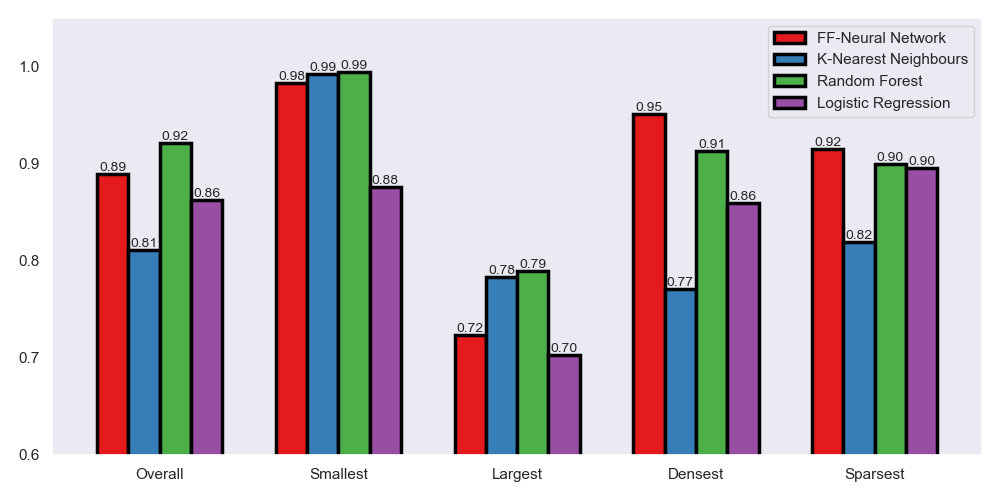
\includegraphics[width=\linewidth]{Images/AUC_ROC.png}
\end{subfigure}
  \hspace*{-1em}
\begin{subfigure}{.45\linewidth}
\vspace*{-1ex}  
\begin{center}
\textbf{Cohen kappa (CK)}
\end{center}
\vspace*{-1ex}
  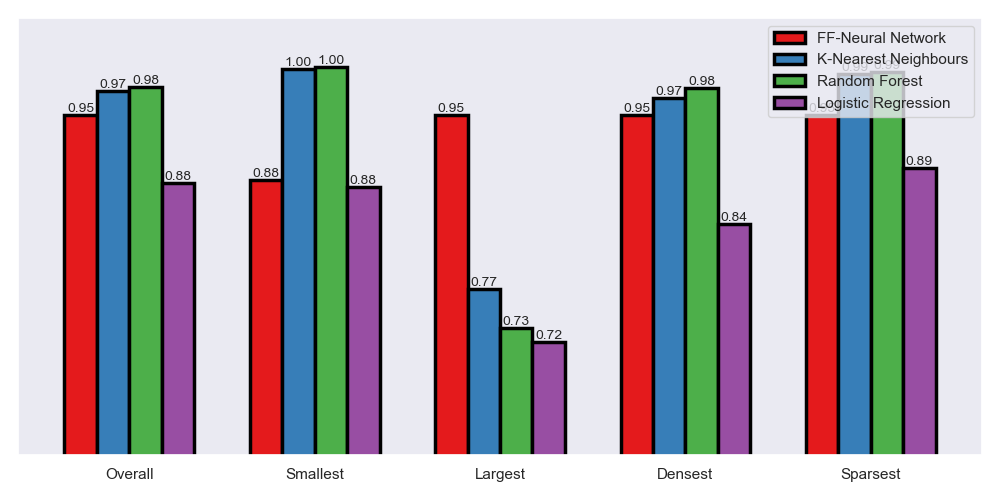
\includegraphics[width=\linewidth]{Images/Cohen_Kappa.png}
\end{subfigure}

\begin{subfigure}{.45\linewidth}
\vspace*{1ex}  
\begin{center}
\textbf{AUC-PR}
\end{center}
\vspace*{-1ex}
  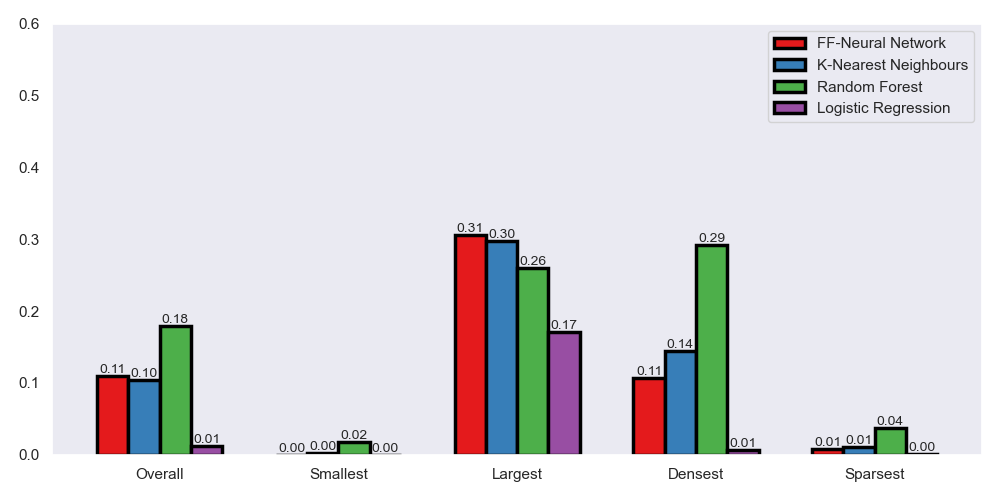
\includegraphics[width=\linewidth]{Images/AUC_PR.png} % f-measure
\end{subfigure}
  \hspace*{-1em}
\begin{subfigure}{.45\linewidth}
\vspace*{1ex}  
\begin{center}
\textbf{F2-measure}
\end{center}
\vspace*{-1ex}
  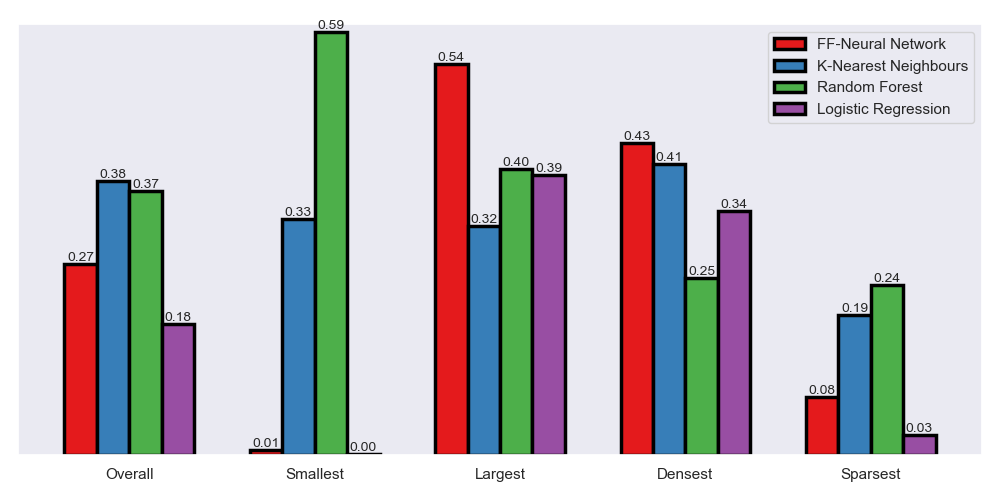
\includegraphics[width=\linewidth]{Images/F2 totals.png} % cohens kappa
\end{subfigure}


\caption{Model performance according to different population distribution types. For each population distribution type the top-5 were evaluated. Note the y axis range for AUC-ROC and Cohen's Kappa (0.6 - 1.0) as opposed to the range for AUC-PR and F-measure  (0.0 - 0.6).}
\label{fig:analysis}
\end{figure}

\subsection{Analysis \& results}

%From figure \ref{fig:analysis}, we see that models tend to achieve better AUC-ROC values with data that has a smaller distribution compared to larger distributions. The opposite is shown with the AUC-PR scores. This is because of the inherent imbalance in the test data; the smallest distributions were attributed to species in the data-set which had very low counts, for example, \emph{Gallotia Stehlini} had only 2 data-points. This skews the Precision and Recall to 0, as well as the False Positive Rate (increasing the ROC score). A variation is not observed between densest and sparsest for the ROC curves, but the densest distribution outperforms the PR score of the sparsest distribution. \hl{This is expected as dense distributions are easier to model/predict?}
From Figure \ref{fig:analysis}, we see that models tend to achieve better AUC-ROC values with data that has a smaller distribution compared to larger distributions. However, the opposite is found with the AUC-PR scores. This is because of the inherent imbalance in the test data; the smallest distributions were attributed to species in the data-set which had very low counts, for example, \emph{Gallotia Stehlini} (35990) had only 2 data-points. This skews the Precision and Recall to 0, as well as the False Positive Rate (increasing the ROC score). A variation is not observed between densest and sparsest for the ROC curves, but the densest distribution outperforms the PR score of the sparsest distribution. This result is expected as denser distributions are generally easier to model due to the data being highly correlated, kin to having fewer `outliers' \cite{ackerman2020detection}. The values for CK are all high, confirming the reliability of our models. The F2-score shows variability in performance between models and between the different distribution types, for example RF and KNN perform consistently well across all types yet FFNN and LR perform comparatively worse on the smallest and sparsest distributions. A visual exploration of results provides a more intuitive evaluation of our models' capabilities to predict species distributions (Figure \ref{fig:map}).

\vspace{-2ex}
\begin{figure}[hbt!]

\centering
\vspace*{-1ex}  
\begin{center}
\textbf{True distribution (test data-set)}
\end{center}
\vspace*{-1ex}
\begin{subfigure}{.3\linewidth}
  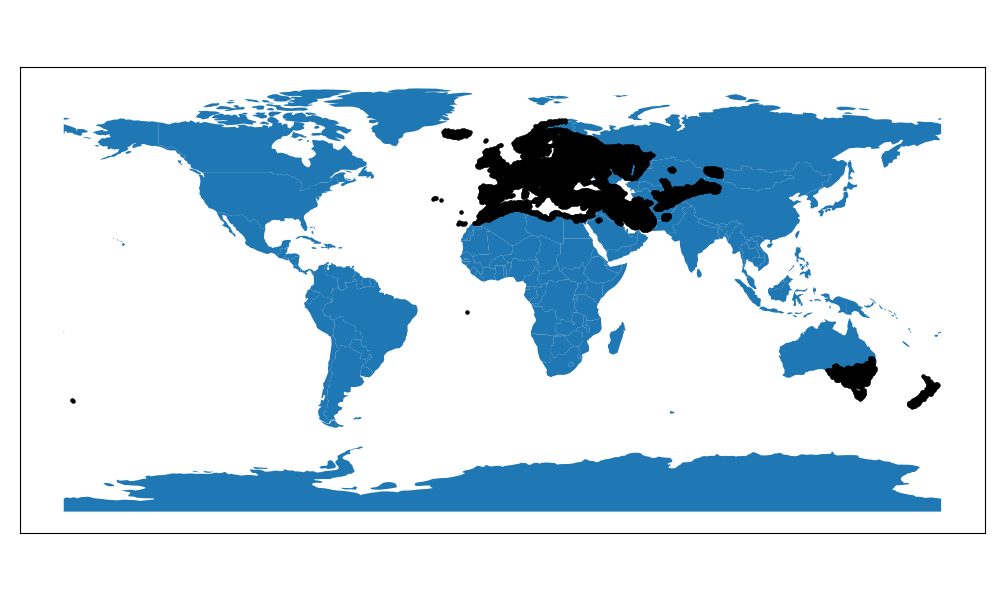
\includegraphics[width=\linewidth]{Images/turdus_true.png}
\end{subfigure} 
\vspace{-3ex}

\begin{subfigure}{.23\linewidth}
  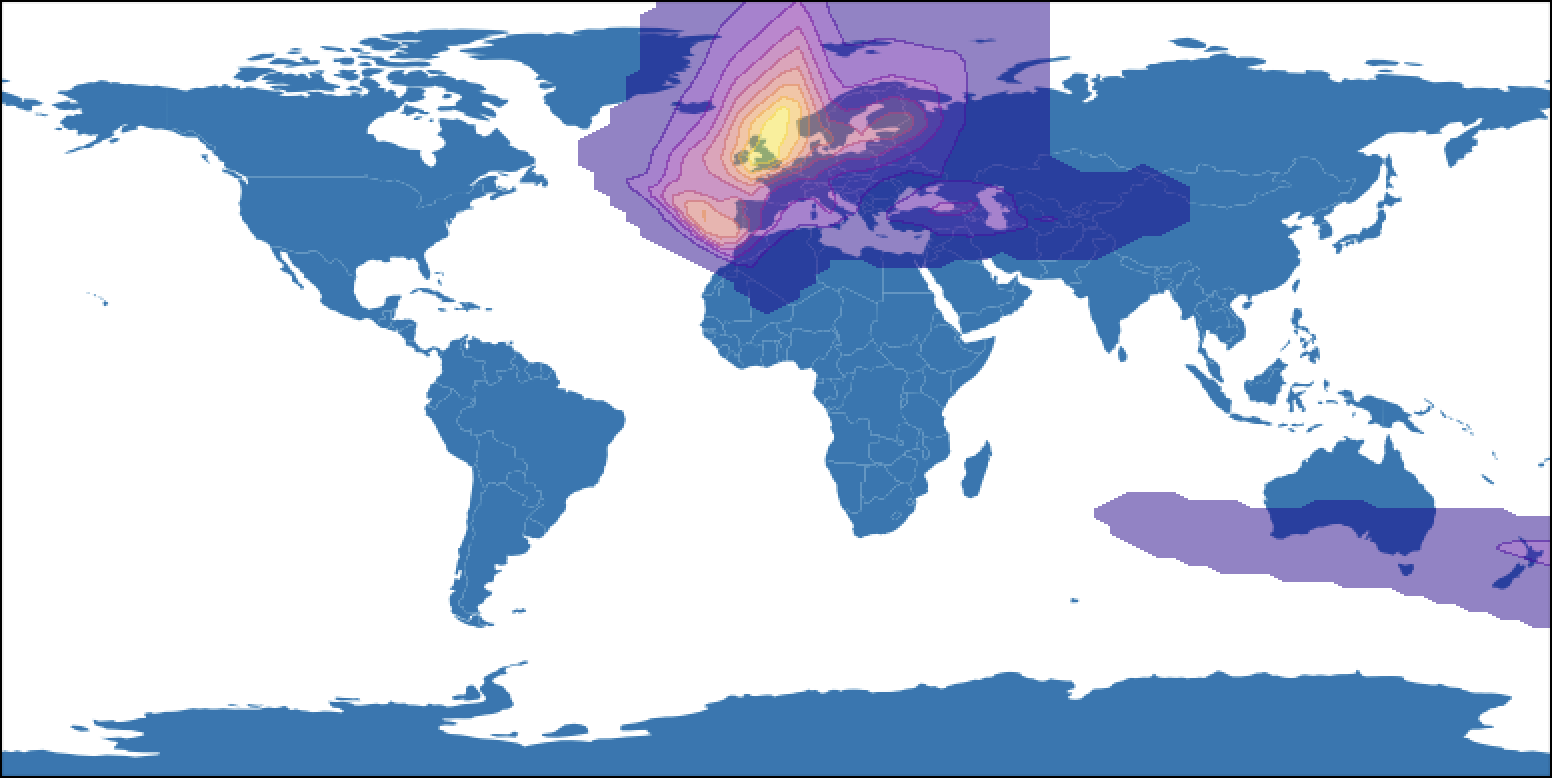
\includegraphics[width=\linewidth]{Images/Screenshot 2023-11-15 at 15.16.04.png}
\vspace*{-3ex}  
\begin{center}
\textbf{Feed-Forward NN}
\end{center}
\end{subfigure}
\begin{subfigure}{.23\linewidth}
  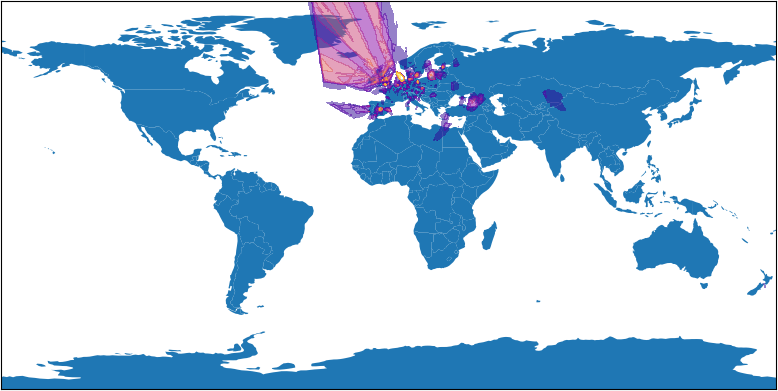
\includegraphics[width=\linewidth]{Images/knn_prediction.png}
\vspace*{-3ex}  
\begin{center}
\textbf{K-Nearest Neighbour}
\end{center}
\end{subfigure}
\begin{subfigure}{.23\linewidth}
  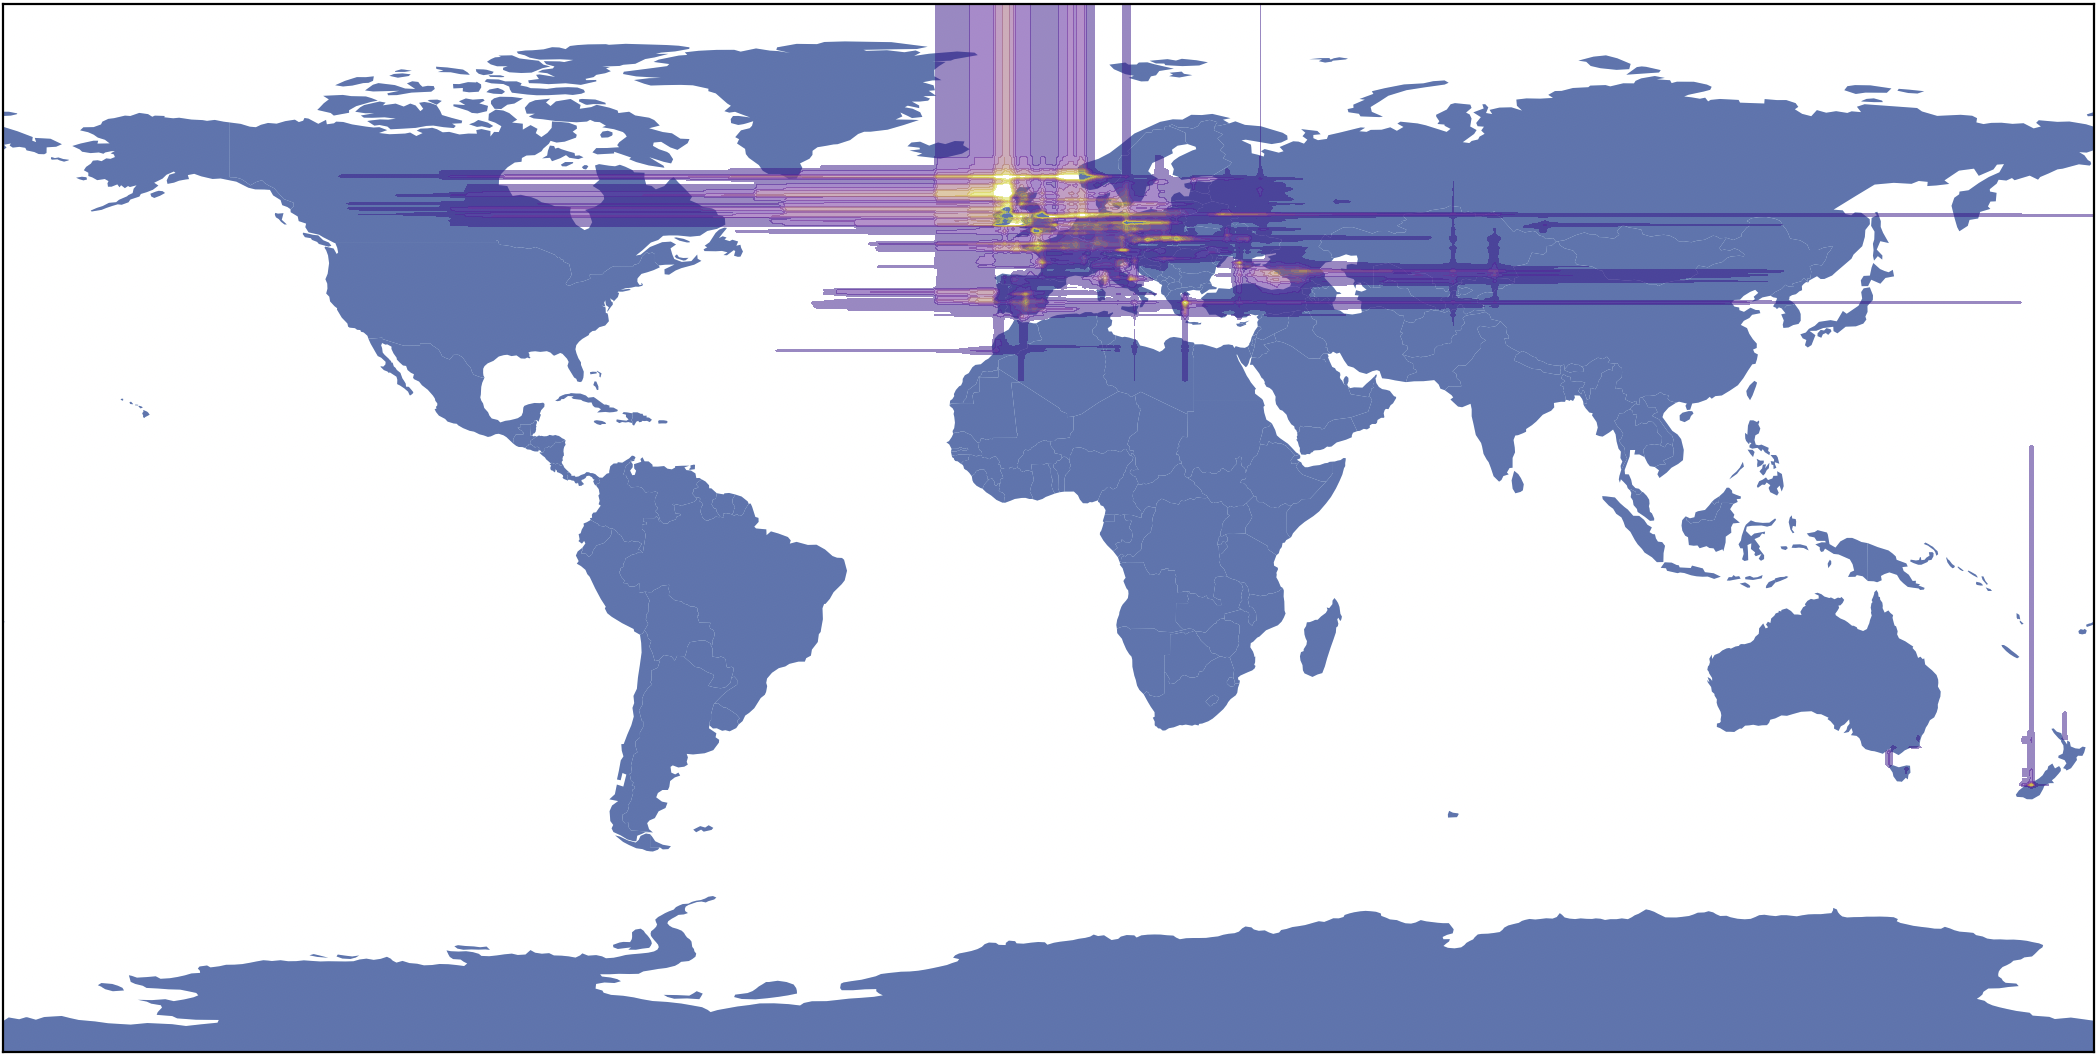
\includegraphics[width=\linewidth]{Images/RFcorrected.png} 
\vspace*{-3ex}  
\begin{center}
\textbf{Random Forest}
\end{center}
\end{subfigure} % <-- "\hfill"
\begin{subfigure}{.23\linewidth}
  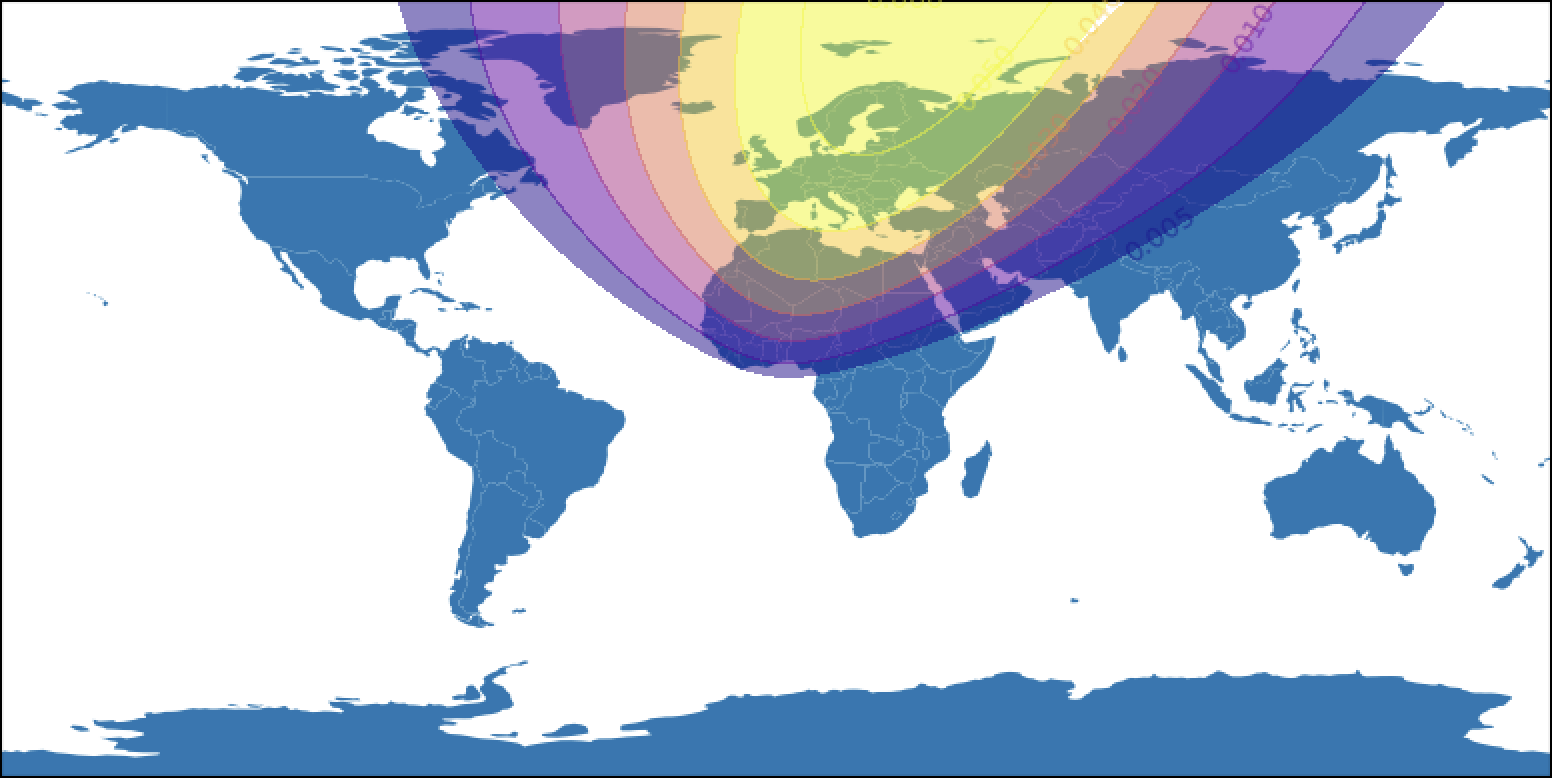
\includegraphics[width=\linewidth]{Images/Screenshot 2023-11-15 at 14.59.56.png}
\vspace*{-3ex}  
\begin{center}
\textbf{Logistic Regression}
\end{center}
\end{subfigure}
\begin{subfigure}{.04\linewidth}
  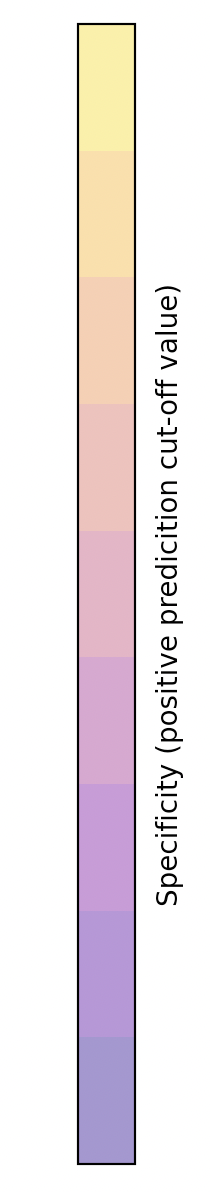
\includegraphics[width=\linewidth, height = 2.5cm]{Images/Screenshot 2023-11-19 at 12.10.01.png}
\end{subfigure}


\caption{Predicted Turdus Merula distributions using various trained models (bottom left-right) vs.\ true distribution (top). Note: The heat-plot nature of the maps is distribution predictions at different model parameters i.e. varying prediction `cut-off' values.}
\label{fig:map}
\end{figure}


%From figure \ref{fig:analysis}, we see that models tend to achieve better AUC-ROC values with data that has smaller distributions compared to larger distributions \hl{why - same reason as the AUC PR, FPs will be way way less likely than TNs hence a FPR close to 0 for classes with small number of locations, this also explains the difference in the axes, can exlain them together in the next paragraph}. A variation in AUC-ROC is not observed in comparing dense vs sparse populations.

%The AUC-PR values indicate the opposite, where larger values for AUC-PR are found in both largely distributed species and densely populated species, whereas small distributions and sparse distributions attain low scores. This is because of the inherent imbalance in the data, the smallest and sparsest distributions were attributed to species in the data-set which had very low counts for example, \emph{Gallotia stehlini} (35990) the species with the smallest distribution had only 2 data points. 

%As a result of the discrepancy between AUC-ROC and AUC-PR values, F-scores and Cohen's Kappa measures were also evaluated. \hl{Here we could mention that results were similar but the NN generally outperforms the other models, to justify its use for the following sections?}

\subsection{Conclusion}

% \hl{Investigating different models' responses to different types of population distribution in the data-set unveiled best AUC-ROC performance for smaller-sized population distributions, however, this was coupled with the worst found AUC-PR scores. The opposite was true for the largest-sized population distributions.- already mentioned?} 
Analyzing our models it is clear that some models are more adept at predicting different population distributions. RF and KNN performed better on average with small and sparse distributions, whereas FFNN performed better with larger distributions.
The Random Forest algorithm consistently did best averaged over all species (0.92, 0.18, 0.99, 0.37 for AUC-ROC, AUC-PR, CK, and F2-score respectively), importantly, however, all models returned very low AUC-PR values. To mitigate our models collective, consistently low AUC-PR results over all population distributions, we further investigate the addition of eight bio-climatic variables into the KNN, FFNN and RF algorithms and their response to the F2 metric.
% \footnote{\hl{The F2 metric specifically considered as we consider the importance of high precision and recall for the problem of SDM. - already mentioned?}}.


\section{Extended analysis of the effect of climate change on different species}

\subsection{Introduction of six new features}

Having been able to classify species at specific locations we now seek to implement new bio-climatic features to improve the prediction capabilities of our models. Annual temperature range, mean temperature of coldest quarter, mean temperature of warmest quarter, annual precipitation, precipitation of driest month, and precipitation seasonality data were sourced for all the locations in the train and test data-sets using WorldClim bio-climatic variables \cite{worldclim}, available at \url{https://www.worldclim.org/data/worldclim21.html}. Figures of these variables can be found in Appendix (\ref{appendix:bio}). Specifically, these new features allow models to produce more accurate results by isolating species predictions within ranges the species can tolerate, for example features like precipitation of driest month can help identify population distributions of desert-based species. The data sourced is restricted to land based, positive-only measurements. As a result, we reduce the task to only consider training for land based species, reducing the train data-set size to 271270. Future work could incorporate marine-based variables such as sea temperature, salinity, and ice content to build a more robust classifier capable of predicting the distribution of marine species in addition to terrestrial species. The Bio-ORACLE data-set \cite{oracle1} \cite{oracle2} would be suitable for this task. Each location data point within the training and test data-sets was combined with the six bio-climatic variables mentioned above, increasing the number of input features to eight. Upon training the models with the newly sourced features, an analysis of the models' F2 scores - specifically chosen due to sensitivity to precision and recall values - was evaluated, shown in Figure \ref{fig:8_feature}.

% \begin{figure}[htp]
% \centering
% \begin{tabular}{@{}c@{}}
% \subfloat{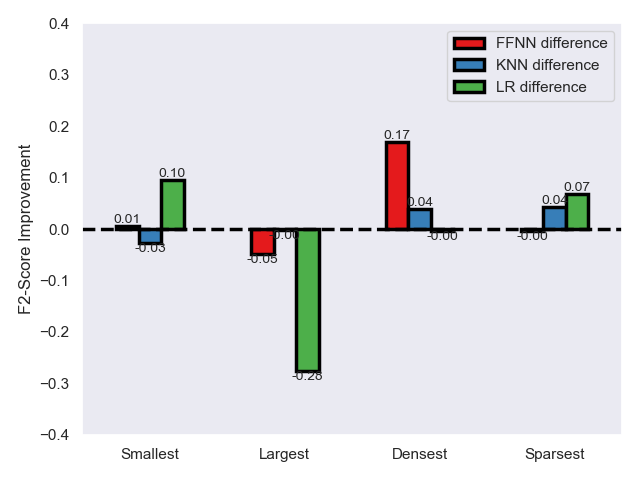
\includegraphics[width=0.4\linewidth]{Images/8_feature_improvement_preemptive.png}}\\
% \end{tabular} % some space
% \begin{tabular}{@{}c@{}}
% \subfloat{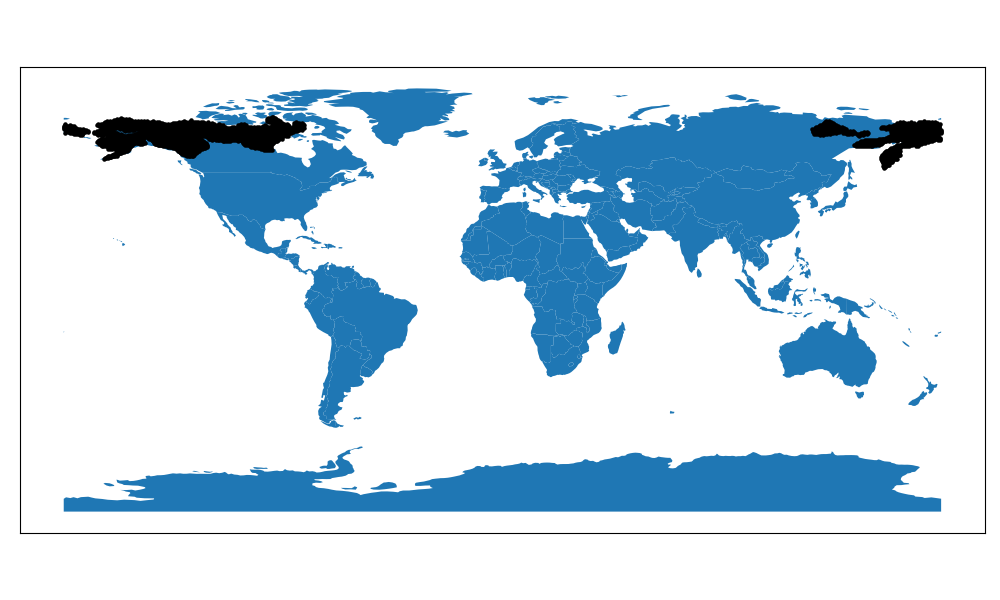
\includegraphics[width=0.25\linewidth]{Images/arctic squirrel true.png}}\\
% \subfloat{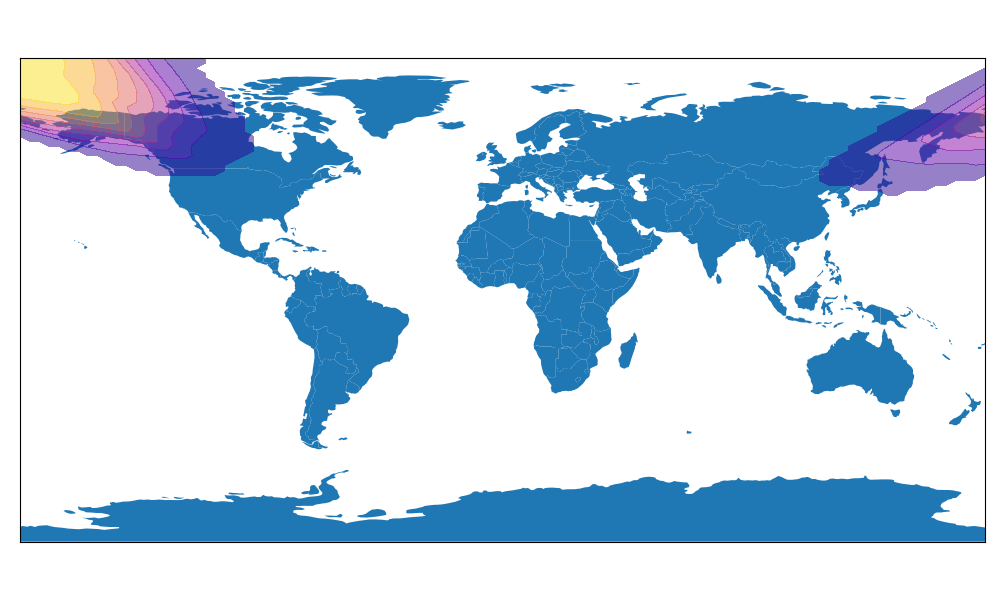
\includegraphics[width=0.25\linewidth]{Images/arctic squirrel 2 feature.png}}
% \subfloat{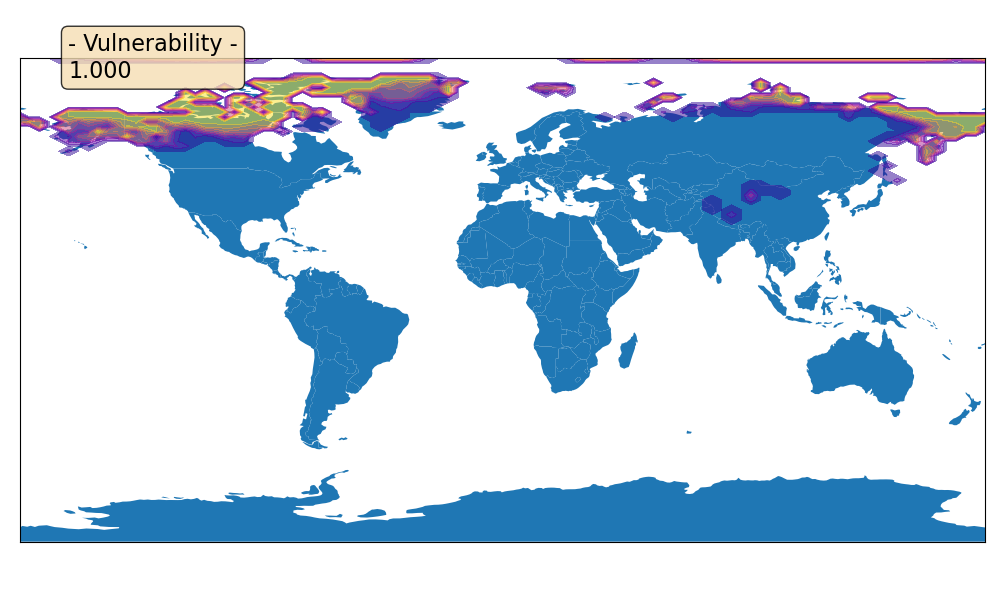
\includegraphics[width=0.25\linewidth]{Images/arctic squirrel vulnerability.png}}
% \\ 
% \end{tabular}
% \caption{Caption.}
% \end{figure}

\begin{figure}[hbt!]
\centering

\begin{subfigure}{.45\linewidth}
\vspace*{-1ex}  
\begin{center}
\textbf{F2 change; 2 feature vs 8 feature}
\end{center}
\vspace*{-1ex}
  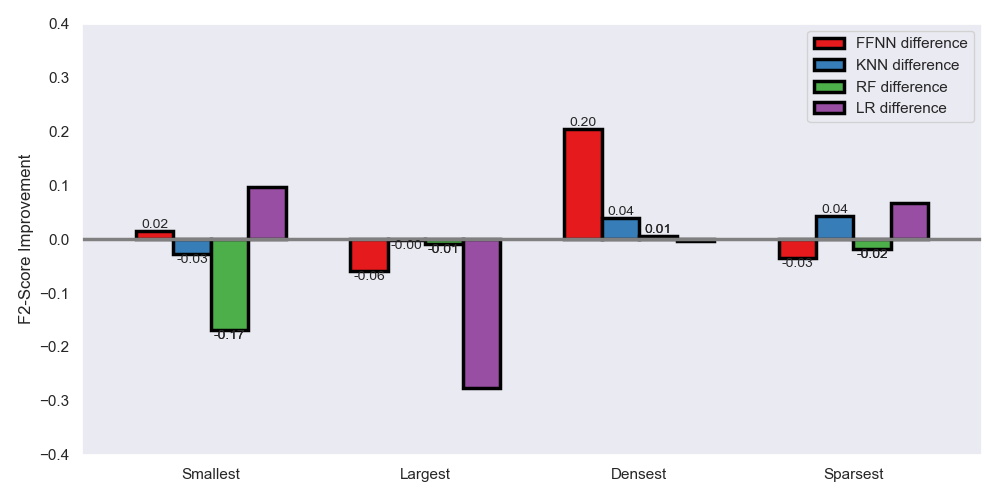
\includegraphics[width=\linewidth]{Images/F2 improvement.png}
\end{subfigure} \hspace{1em}  % <-- "\hfill"
\begin{subfigure}{.3\linewidth}
  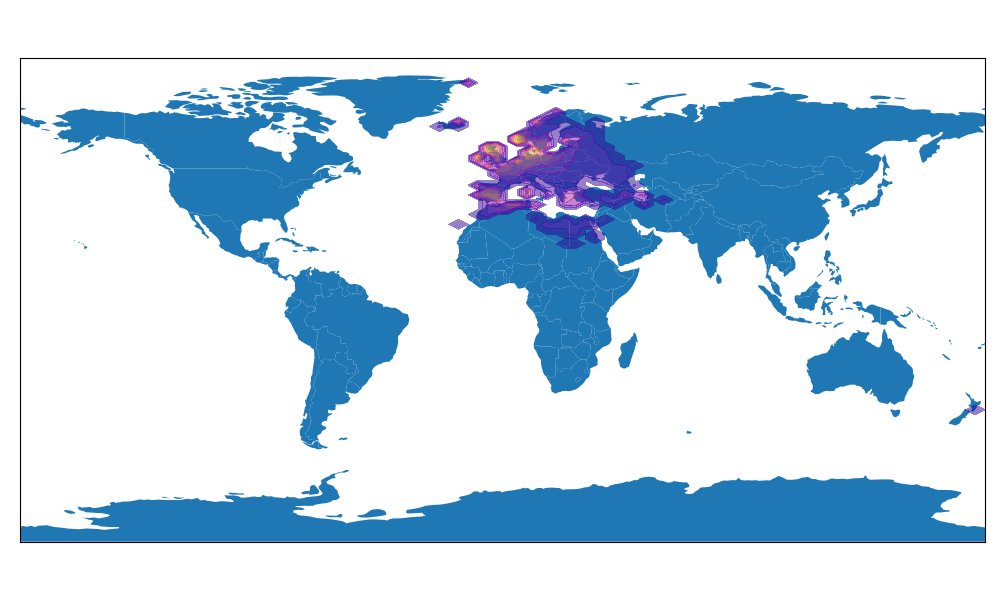
\includegraphics[width=\linewidth]{Images/8 feature turdus.png}
\vspace*{-5ex}  
\begin{center}
\textbf{FFNN-8 feature Turdus Merula}
\end{center}
\vspace{0ex}
\end{subfigure}
\begin{subfigure}{.04\linewidth}
  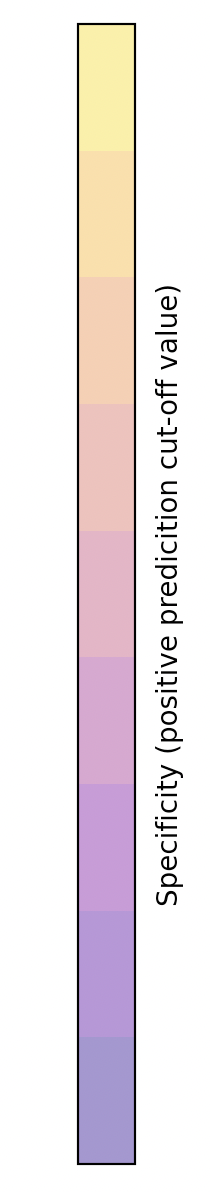
\includegraphics[width=\linewidth, height = 2.5cm]{Images/Screenshot 2023-11-19 at 12.10.01.png}
  \vspace{1ex}
\end{subfigure}

\caption{(Left) The metric improvements/losses when trained with new 8-feature data (land-based species only). (Right) Newly predicted Turdus Merula distribution from the FFNN (most improved).}
\label{fig:8_feature}
\end{figure}
As can be seen from Figure \ref{fig:8_feature}, the FFNN model experienced the biggest improvements. Notably, the models performed worse on some types of population distribution; this is because the new features help identify similar regions to that input, smaller distributed populations are then over-identified in a broader range of regions that would be `climatically suitable', as shown in appendix \ref{appendix:smalldistn}. Additionally, introducing 6 new features may have led to overfitting of the data, explaining the overall lower than expected improvement in F2 score.



% Figure \hl{X} shows the changes in accuracy of species distribution prediction with the introduction of the new features...

% A visual comparison of a predicted species distribution, \emph{Oenanthe leucopyga}, is shown in figure \ref{fig:extra_feature}

% \emph{Oenanthe Leucopyga} is known to inhabit desert, rocky areas; resident to the sahel regions in Africa, stretching into parts of the middle east \hl{cite}. The original models trained on 2-features fail to capture this behaviour, incorrectly predicting exact population distributions. The 8-feature trained models manage to capture population distributions by extending predictions beyond given limited location data into regions which would be suitable for species based on given location bioclimatic variables.


\subsection{Effect of climate change on newly trained models}
We now use a FFNN, combined with the new bio-climatic features, to predict species most at risk due to climate change. To quantify the effects of climate change, we examine the difference in yearly average temperatures between a baseline value, calculated as the mean over 30 years from 1984-2014, and a projected value for the year 2050, computed under the high emissions scenario (SSP5-8.5). The temperature data is taken from the Met Office Hadley Centre HadGEM3-GC31-LL model \cite{met}, prepared for the Coupled Model Intercomparison Project Phase 6 (CMIP6). A visualization of temperature anomaly is shown in appendix \ref{appendix:temp-anomaly}. Based on the 2050 temperature anomaly, we now compute a "score" that quantifies how extreme the predicted temperature increase of a particular location will be due to climate change, which is obtained by normalising the temperature anomaly by the largest increase (in this case 17$^\circ$C). We note that a few localised patches of ocean saw a decrease in yearly temperatures based on the model data, however, since these areas were small and the decrease was less than a degree, we set the temperature anomaly for these locations to 0$^\circ$C for the purposes of calculation. Combining this analysis of climate data at different locations with our models' improved prediction capability we can now provide accurate population distribution predictions and a `vulnerability' score for specific species as shown in Table \ref{tab:vulnerability}. We note that our vulnerability score is quite simplistic in the sense that a larger increase in temperature does not necessarily translate to a larger negative effect on a species, for example, certain species might be more resilient to changes in temperature than others. For future work, we might define this score differently by considering multiple climate metrics in addition to the yearly average temperature anomaly, for example, the anomalies in maximum temperature of the warmest month, lowest temperature of the coldest month, precipitation rates, sea ice content, etc. This would give a more complete evaluation of how climate change affects habitats beyond an increase in yearly average temperatures. Notably, species with high vulnerability were located near the poles (latitudes of $\approx 80$ and $\approx-80$ for the Arctic Ground Squirrel, shown in appendix \ref{appendix:arcticsq} and Chinstrap Penguin respectively), whereas species with low vulnerability were located in temperate regions between $\approx-50$ and $\approx-60$ latitude.


\begin{table}[hbt!]
\begin{tabular}{ |p{2cm}|p{2cm}|p{2cm}||p{2cm}|p{2cm}|p{2cm}|  }
 \hline
 \multicolumn{6}{|c|}{\textbf{Climate change vulnerability analysis}} \\
 \hline
 \rowcolor{lightgray} \footnotesize{\textbf{Most Vulnerable}}& \footnotesize{\textbf{Vulnerability}} & \footnotesize{\textbf{Location (largest pop.)}} & \footnotesize{\textbf{Least Vulnerable}} & \footnotesize{\textbf{Vulnerability}} & \footnotesize{\textbf{Location (largest pop.)}} \\
 \hline
\scriptsize{\emph{Arctic G. Squirrel}}  & \scriptsize{1.0 (298.15)} & \scriptsize{N.America} & \scriptsize{\emph{Black Rain Frog}} & \scriptsize{0.000002} & \scriptsize{Africa} \\
\scriptsize{\emph{Chinstrap Penguin}} & \scriptsize{0.70}  & \scriptsize{Antarctica} & \scriptsize{\emph{Whistling Tree Frog}} & \scriptsize{0.000012} & \scriptsize{Australia} \\
\scriptsize{\emph{Pine Grosbeak}} & \scriptsize{0.38} & \scriptsize{N.America} & \scriptsize{\emph{Golden C. Snake}} & \scriptsize{0.000012} & \scriptsize{Australia} \\
\scriptsize{\emph{Common Redpoll}} & \scriptsize{0.20} & \scriptsize{Europe}  & \scriptsize{\emph{Cape Mole Rat}} & \scriptsize{0.000015} & \scriptsize{Africa} \\
\scriptsize{\emph{Ruffed Grouse}} &  \scriptsize{0.18}  & \scriptsize{N.America} & \scriptsize{\emph{Tusked Frog}} & \scriptsize{0.000016} & \scriptsize{Australia} \\

 \hline
\end{tabular}
\caption{An analysis of the most and least vulnerable species to climate change. Scores were scaled according to that achieved by the most vulnerable species.}
\label{tab:vulnerability}
\end{table}
\vspace{-3ex}
